%% trackmeasure paper draft -- ACM AsiaCCS format (acmart, sigconf).
%% Submission: switch to [sigconf,review,anonymous] (double-blind) and check the
%% current AsiaCCS CFP for page limits and the exact \acmConference values.
%% Red [TBD: ...] marks every number or claim that needs real data. Do not remove a
%% TBD without replacing it with a measured value from results/.
\documentclass[sigconf,review,anonymous]{acmart}

\usepackage{tikz}
\usetikzlibrary{positioning,arrows.meta,fit}

\setlength{\emergencystretch}{2em}
\newcommand{\TBD}[1]{\textcolor{red}{[TBD: #1]}}
\newcommand{\NOTE}[1]{\textcolor{blue}{[Note: #1]}}
\newcommand{\sys}{\textsc{TrackMeasure}}

%% ---- Front-matter placeholders (replace with values from the CFP) ----
\setcopyright{none}
\acmConference[AsiaCCS '27]{ACM Asia Conference on Computer and Communications Security}{TBD}{TBD}
\acmYear{2027}
\settopmatter{printacmref=false}
\renewcommand\footnotetextcopyrightpermission[1]{}

\begin{document}

\title{Does Opting Out Stop Fingerprinting? Measuring Advanced Tracking, Blockers and Consent on Popular Websites}

% Authors withheld for now (anonymous draft). Add real authors and drop `anonymous` later.
\author{Anonymous Author(s)}
\affiliation{\institution{Anonymous Institution}\city{Anonymous}\country{Anonymous}}
%% TODO: add remaining group members; remove names (and use [anonymous]) for double-blind submission.

\begin{abstract}
Browser fingerprinting, behavioural-signal collection and cookie respawning let websites and
third parties recognise users without, or despite, the cookies that consent banners and
privacy tools are designed to control. We present \sys{}, an instrumented, containerised
crawler that attributes calls to about 70 fingerprinting-, storage- and input-related browser
APIs to the script that made them and, unlike API-level measurements, checks whether the
computed fingerprint values and identifiers actually leave the browser and to whom. We replay
an identical browsing flow on \TBD{N} popular news, e-commerce and social/affiliate websites
under repeated baselines, two Manifest~V3 blockers, consent rejection and Global Privacy Control
(separately and combined), and acceptance. We count an opt-out only when the consent manager's
own state confirms it, and we classify pay-or-OK walls separately. We find that \TBD{X\%} of
sites run fingerprinting scripts, \TBD{Y\%} before any consent interaction, and that
fingerprint values reach \TBD{E} third-party domains. After a verified rejection,
\TBD{Z\%} of fingerprinting (script, technique) pairs and \TBD{Z$_e$\%} of exfiltration
flows persist, which is \TBD{not / significantly} different from the variation between two
identical crawls. Blockers reduce them to \TBD{B\%}. A three-browser protocol identifies
\TBD{R} sites whose identifiers respawn after cookies are cleared, \TBD{F} of them from the
fingerprint alone.
\end{abstract}

\begin{CCSXML}
<ccs2012>
<concept><concept_id>10002978.10003022.10003026</concept_id>
<concept_desc>Security and privacy~Web application security</concept_desc>
<concept_significance>500</concept_significance></concept>
<concept><concept_id>10002978.10003029.10011150</concept_id>
<concept_desc>Security and privacy~Privacy protections</concept_desc>
<concept_significance>300</concept_significance></concept>
</ccs2012>
\end{CCSXML}
\ccsdesc[500]{Security and privacy~Web application security}
\ccsdesc[300]{Security and privacy~Privacy protections}
\keywords{browser fingerprinting, web measurement, consent management platforms, cookie respawning, ad blockers, Global Privacy Control, pay-or-OK}

\maketitle

%% ======================================================================
\section{Introduction}
%% ======================================================================
Cookie banners and content blockers give users the impression of control over web tracking.
Both, however, are built around third-party requests and stored identifiers. Stateless
techniques such as canvas, audio and WebRTC fingerprinting~\cite{mowery2012pixel,eckersley2010unique,laperdrix2020survey}
need neither, and stateful identifiers can be rebuilt from a fingerprint after the user deletes
them~\cite{acar2014web,fouad2022phoenix}. Recent work reports that fingerprinting continues after
users opt out~\cite{liu2025fptrace}, while measurements of consent banners show that recorded
choices frequently diverge from what users selected~\cite{matte2020cookie,nouwens2020dark}.

Three gaps make these effects hard to quantify. First, most crawls treat a click on a
``Reject all'' button as an opt-out without checking that the consent manager registered it,
so tracking that ``survives'' a rejection may simply mean the rejection never happened.
Second, API-level detection shows that a script \emph{computed} a fingerprint, not that the
value was \emph{sent} anywhere; benign uses such as bot detection call the same APIs.
Third, blocker evaluations largely predate Chromium's move to Manifest~V3, which restricts
what extensions such as uBlock Origin can do~\cite{chromemv3}.

We ask four questions:
\begin{description}
\item[RQ1] How prevalent are fingerprinting, behavioural-signal collection, identifier sharing
  and storage abuse on popular news, e-commerce and social/affiliate websites, how much happens
  before consent, and which parties receive fingerprint values?
\item[RQ2] How much fingerprinting, and how much fingerprint exfiltration, survives a
  Manifest~V3 blocker (uBlock Origin Lite, Privacy Badger)?
\item[RQ3] Does a \emph{verified} consent rejection stop it, does Global Privacy
  Control~\cite{gpcspec}, and do they combine? Acceptance serves as the upper bound.
\item[RQ4] Do identifiers respawn after cookies are cleared, and can they be re-derived from
  the browser fingerprint alone?
\end{description}

\paragraph{Contributions.}
\begin{itemize}
\item \sys{}, an open, containerised measurement pipeline that runs one fresh browser profile
  per site through an identical four-phase flow under nine conditions, with per-call script
  attribution for about 70 APIs (\S\ref{sec:method}).
\item Value-level evidence: we capture the canvas and WebGL values scripts compute and search
  for them, raw or hashed, in outgoing requests, and track identifier-like cookie values sent to
  other parties (\S\ref{sec:value}).
\item A consent-verification procedure that reads IAB TCF~v2~\cite{iabtcf} and Cookiebot state
  across frames, re-checks it after reload and on subpages, excludes unverified choices, and
  separates pay-or-OK walls from automation failures (\S\ref{sec:consent}).
\item A measurement on \TBD{N} sites reporting prevalence, blocker and opt-out effects as paired
  differences against a measured noise floor, manually validated detector precision, and
  stateful versus fingerprint-derived respawning (\S\ref{sec:results}).
\end{itemize}

%% ======================================================================
\section{Background and Related Work}
%% ======================================================================
\paragraph{Fingerprinting.} Eckersley showed that browser attributes alone identify most
users~\cite{eckersley2010unique}; canvas rendering differences add further
entropy~\cite{mowery2012pixel}. Large crawls documented canvas, font, WebRTC and audio
fingerprinting in the wild~\cite{acar2013fpdetective,acar2014web,englehardt2016online}, and
FP-Inspector combined static and dynamic analysis to detect fingerprinting
scripts~\cite{iqbal2021fingerprinting}. We adopt the Englehardt--Narayanan detection
heuristics~\cite{englehardt2016online} as refined by FP-Inspector, and add two weaker signals.
Laperdrix et al.\ survey the field~\cite{laperdrix2020survey}. Behavioural signals (mouse,
keyboard, touch and motion-sensor data) can also identify users
\TBD{cite behavioural-biometrics work, verified}, but their collection by third-party scripts is
rarely measured at scale.

\paragraph{Effects, not only API use.} Static or API-level detection cannot tell fingerprinting
from benign uses of the same APIs. FPTrace instead links fingerprint changes to ad-bidding
outcomes and reports that fingerprinting persists after opt-out~\cite{liu2025fptrace}. Cookie
syncing, i.e.\ identifiers passed between trackers, has been measured by matching identifier
values in request URLs~\cite{acar2014web,papadopoulos2019cookiesync}. We apply value matching to
fingerprint values themselves.

\paragraph{Respawning.} Acar et al.\ measured respawning through Flash cookies and
storage~\cite{acar2014web}; Fouad et al.\ showed that cookies can be respawned from browser
fingerprints~\cite{fouad2022phoenix}. Our three-browser protocol separates the two mechanisms.

\paragraph{Consent.} Consent management platforms (CMPs) spread rapidly after the
GDPR~\cite{hils2020cmp}. Their interfaces often nudge acceptance~\cite{nouwens2020dark}, and
stored TCF consent strings do not always match user choices~\cite{matte2020cookie}.
Automated consent handling has been used to detect violations at scale~\cite{bollinger2022cookieblock}.
Pay-or-OK walls, where the only alternative to consenting is a subscription, are spreading
among news publishers \TBD{cite pay-or-OK measurement, verified}.

\paragraph{Blockers and evasion.} Filter-list blockers are evaluated against trackers
in~\cite{merzdovnik2017block}; CNAME cloaking lets third-party trackers appear
first-party~\cite{dimova2021cname}. Manifest~V3 replaces blocking web-request listeners
with declarative rules~\cite{chromemv3}; we measure the MV3 builds users now receive.

%% ======================================================================
\section{Methodology}\label{sec:method}
%% ======================================================================

\begin{figure}[t]
\centering
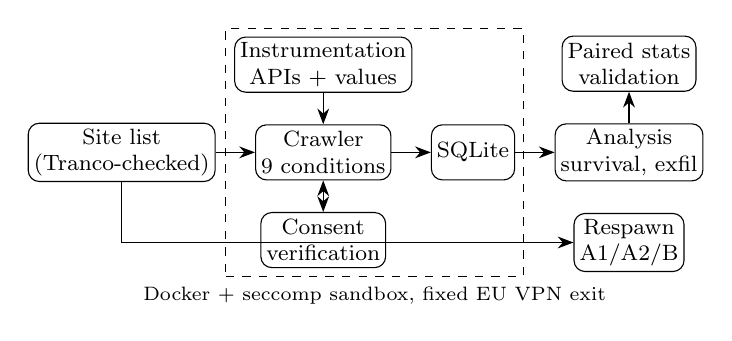
\begin{tikzpicture}[node distance=4mm and 5mm, font=\footnotesize,
  box/.style={draw, rounded corners, align=center, minimum height=7mm, inner sep=2pt},
  >={Stealth[length=2mm]}]
\node[box] (sites) {Site list\\(Tranco-checked)};
\node[box, right=of sites] (crawl) {Crawler\\9 conditions};
\node[box, above=of crawl] (inst) {Instrumentation\\APIs + values};
\node[box, below=of crawl] (cons) {Consent\\verification};
\node[box, right=of crawl] (db) {SQLite};
\node[box, right=of db] (an) {Analysis\\survival, exfil};
\node[box, below=of an] (resp) {Respawn\\A1/A2/B};
\node[box, above=of an] (st) {Paired stats\\validation};
\draw[->] (sites) -- (crawl); \draw[->] (inst) -- (crawl); \draw[<->] (cons) -- (crawl);
\draw[->] (crawl) -- (db); \draw[->] (db) -- (an); \draw[->] (an) -- (st);
\draw[->] (sites.south) |- (resp.west);
\node[draw, dashed, inner sep=3pt, fit=(inst)(cons)(crawl)(db),
  label={[font=\scriptsize]below:Docker + seccomp sandbox, fixed EU VPN exit}] {};
\end{tikzpicture}
\Description{Block diagram: the site list feeds the crawler, which is driven by the instrumentation and consent verifier and writes to SQLite; SQLite feeds the analysis, which feeds paired statistics and validation; the site list also feeds the respawn experiment. The crawler components sit inside a dashed box labelled Docker with seccomp sandbox and fixed EU VPN exit.}
\caption{\sys{} pipeline. All browsing runs inside a sandboxed container whose traffic leaves
through a single, fixed VPN exit.}
\label{fig:pipeline}
\end{figure}

\subsection{Site selection}
We seed \TBD{150} sites, 50 each in news/media, e-commerce and social/affiliate, and check them
against the Tranco list~\cite{lepochat2019tranco} (list ID \TBD{ID}, downloaded \TBD{date}).
We drop sites outside the top \TBD{rank}, sites that redirect to another registrable domain,
and sites that fail in the baseline. Because only TCF and Cookiebot states can confirm a
choice (\S\ref{sec:consent}), we \TBD{ensure at least $k$ sites per category expose one of
them, so that the opt-out comparison is not limited to a handful of sites; state the rule}.

\subsection{Crawl procedure}
Each site is visited with a fresh Chromium profile (Playwright~1.63, Chromium~\TBD{version
from run metadata}) through four phases that are identical in every condition:
\emph{landing} (homepage, no banner interaction), \emph{after\_consent} (the condition's
consent action, or none), \emph{home\_reload} (homepage reloaded with the stored consent
state) and \emph{subpage}~$\times n$ (same-site links chosen in the baseline and reused in
every later condition). On each page the crawler scrolls and moves the mouse for a fixed dwell
time. Settings: \TBD{headful/Xvfb, workers, dwell, $n$ subpages, timeouts, locale,
timezone; must be identical across conditions}. A visit counts as complete only with a
successful HTTP document response and a DOMContentLoaded event; any failed visit invalidates
the site/run for comparisons.

\paragraph{Instrumentation.} An init script, injected into every frame before page scripts
run, wraps about 70 APIs: canvas 2D and WebGL, Web Audio, WebRTC, navigator and screen
getters, font checks, \texttt{matchMedia}, Web Storage, IndexedDB, \texttt{document.cookie} and
\texttt{sendBeacon}. It also records canvas \texttt{save}/\texttt{restore} calls and canvas event
listeners (for the animation exclusion below), registrations of behavioural listeners
(pointer, keyboard, touch, wheel/scroll and device-motion events, including \texttt{on*}
properties), and Generic Sensor constructors. Each call is attributed to the calling script
from the JavaScript stack trace and mapped to its registrable domain (eTLD+1). Wrapped
functions return the native \texttt{toString()} text to avoid trivial tamper checks. We also
log every request with its body (up to 64\,KB), whether an extension blocked it, and the
final cookie jar.

\paragraph{Conditions.} Table~\ref{tab:conditions} lists the conditions. They run back to
back from the same VPN exit (Netherlands), reusing baseline subpage URLs. The combined opt-out
and its two components let us attribute an effect to the banner choice, to GPC, or to both.

\begin{table}[t]
\caption{Crawl conditions.}\label{tab:conditions}
\small
\begin{tabular}{@{}lll@{}}
\toprule
Run & Setup & Purpose \\
\midrule
baseline   & plain browser                 & reference \\
baseline2/3 & identical repeats            & noise floor \\
ubol       & uBlock Origin Lite$^\ast$     & MV3 blocker \\
pbadger    & Privacy Badger$^\ast$         & MV3 blocker \\
optout     & verified reject + GPC         & opt-out \\
rejectonly & verified reject               & banner choice \\
gpconly    & GPC, no banner action         & browser signal \\
accept     & verified accept               & upper bound \\
\bottomrule
\end{tabular}\\[2pt]
{\footnotesize $^\ast$uBOL 2026.1110.1816; Privacy Badger 2026.9.15.2 (pinned).}
\end{table}

\paragraph{Blockers.} Both extensions are installed from hash-pinned official Chromium
packages and are not modified. Before each site, the crawler waits until their rules are
ready; a missing or uninitialised extension fails the site instead of crawling unprotected.
uBlock Origin Lite runs in its default \emph{optimal} mode with six default static rulesets.
Privacy Badger uses its bundled seed data with local learning disabled and sends GPC by
default, so its condition measures the extension's full default behaviour, not blocking alone.

\subsection{Consent verification}\label{sec:consent}
For the conditions with a banner action, the crawler first calls the CMP's JavaScript API
(OneTrust, Cookiebot, Didomi, Usercentrics), then falls back to clicking visible controls
whose accessible names match anchored regular expressions in seven languages, including a
two-step ``manage options, then reject/save'' flow. A choice counts as \emph{confirmed} only when
a completed action is followed by readable saved state, either a TCF~v2 event whose purpose
consents match the request or a Cookiebot response with all optional categories matching.
A vanished banner or a successful function call is not sufficient. State is read across the
main page and all frames and re-checked after the reload and on every subpage. Contradictory
reports or lost state downgrade the outcome to \emph{unknown}. Only confirmed site/runs
enter the consent comparisons; Table~\ref{tab:consent} reports all outcomes.

When a rejection fails, we classify the visible controls: an accept control together with a
paid option (``subscribe'', ``abo'', a price per month) and no free reject control is recorded
as \emph{pay-or-OK}. Such sites stay excluded from the opt-out comparison, but are reported as a
site design rather than an automation failure; we confirm each case from a saved screenshot.
GPC is sent as the \texttt{Sec-GPC} header and exposed as \texttt{navigator.globalPrivacyControl};
we record its observed value on the final page.

\subsection{Fingerprinting detection}
We group calls by (visit, frame, script) and flag the techniques in
Table~\ref{tab:heuristics}. The first four follow Englehardt and
Narayanan~\cite{englehardt2016online}, including their exclusion of scripts that animate the
canvas (\texttt{save}/\texttt{restore} or canvas event listeners); \emph{webgl} and
\emph{attr\_enum} are weaker additions that we report separately. To estimate precision, two
authors independently label a stratified random sample of \TBD{15} detected scripts per
technique as fingerprinting or not, resolving disagreements by discussion; we report precision
with Wilson 95\% intervals (Table~\ref{tab:validation}).

\begin{table}[t]
\caption{Fingerprinting heuristics (per script, frame and visit).}\label{tab:heuristics}
\small
\begin{tabular}{@{}lp{0.68\columnwidth}@{}}
\toprule
Technique & Rule \\
\midrule
canvas      & $\geq$10 distinct characters drawn, a non-lossy readback of a canvas $\geq$16$\times$16, no \texttt{save}/\texttt{restore} or canvas listener \\
canvas\_font & \texttt{measureText} with $\geq$50 distinct fonts \\
webrtc      & \texttt{createDataChannel} and \texttt{createOffer} \\
audio       & oscillator, dynamics compressor and a readback \\
webgl       & \texttt{getParameter} of unmasked vendor/renderer \\
attr\_enum  & $\geq$12 distinct navigator/screen attributes read \\
\bottomrule
\end{tabular}
\end{table}

\subsection{Value-level evidence}\label{sec:value}
\paragraph{Fingerprint exfiltration.} For the first ten calls per API and frame, the init
script also returns the value of \texttt{toDataURL} and of WebGL's unmasked vendor and renderer
strings. We store only match tokens, never the image: a 48-character slice of the canvas image
data, the raw and base64-encoded strings, and their MD5, SHA-1 and SHA-256 digests. A
fingerprint is \emph{exfiltrated} when a token appears in the URL (also after URL-decoding) or
body of a later request that the browser actually sent, i.e.\ one not blocked by an extension.
This is a lower bound: values combined with other attributes, or hashed with custom functions
such as MurmurHash, are not recognised.

\paragraph{Identifier sharing.} An identifier-like cookie value ($\geq$10 characters,
containing a digit, varied, not a timestamp) found in a request to a registrable domain other
than the cookie's owner counts as shared. Consent-string cookies (e.g.\ \texttt{euconsent-v2})
are excluded because they are sent to vendors by design.

\paragraph{Behavioural signals.} We count third-party scripts that register listeners from at
least two families (pointer, keyboard, touch, scroll, motion). Registration alone is not proof
of behavioural tracking; we report it together with exfiltration evidence.

\subsection{Metrics and statistics}
For a site $s$ and condition $c$, let $P_{s,c}$ be the set of (script eTLD+1, technique) pairs
detected in the post-consent phases. \emph{Survival} is
\[
  \mathrm{surv}(s,c) = \frac{|P_{s,\mathrm{baseline}} \cap P_{s,c}|}{|P_{s,\mathrm{baseline}}|}.
\]
\emph{Exfiltration survival} is defined in the same way over (receiving eTLD+1, value kind)
pairs. Both are computed over sites where both runs completed and, for consent conditions, the
choice was confirmed. Because ads and scripts rotate between visits, even an identical repeat
does not reach 1. We therefore compare each condition with the noise floor per site: for every
site we take $d_s = \mathrm{surv}(s,c) - \mathrm{surv}(s,\mathrm{baseline2})$ and report the
median $d_s$ with a bootstrap 95\% confidence interval and an exact two-sided sign test. A third
baseline estimates the variability of the noise floor itself. We also report third-party
domains contacted, blocked requests, and fingerprinting observed in the \emph{landing} phase
(before any consent).

\subsection{Respawning}
On a subset of \TBD{M} sites whose baseline set persistent, identifier-like cookies (third
party or $\geq$90-day expiry), we run three browsers from the same IP. \textbf{A1} visits with
profile~A and fingerprint F1. \textbf{A2} revisits with F1 either after deleting cookies only
(\emph{stateful}: the value may be restored from localStorage or IndexedDB) or in a brand-new
profile (\emph{fingerprint-derived}). \textbf{B} visits with a fresh profile and a different
fingerprint F2 (viewport, pixel ratio, locale, time zone, hardware concurrency, device memory,
canvas noise). An identifier-like token from an A1 cookie is respawned if it reappears in an
A2 cookie and nowhere in B; the B control rules out values shared by all users and, with a
fresh profile on the same IP, IP-only keying.

\subsection{Isolation and validation}
The crawler executes untrusted third-party JavaScript, so it runs in a Docker container
inside a VM, as a non-root user, with all capabilities dropped, Playwright's seccomp
profile, and Chromium's own sandbox enabled. Only the data, extension (read-only) and results
directories are mounted. Traffic leaves through a WireGuard VPN container; we verified that
the crawler loses connectivity when the VPN stops. A local fixture with an aggressive
tracker, a consent-respecting tracker, consent failure and pay-or-OK pages, and a test blocker
checks the pipeline end to end. All six techniques are detected. The tracker's canvas and
WebGL values are found in its requests, together with its identifier. Under the blocker,
survival and exfiltration survival are both 0. A consent-ignoring tracker yields opt-out
survival 1, the pay-or-OK page is classified as such, and both respawning mechanisms are
found. Real blockers are checked offline against a locally impersonated tracker domain.

%% ======================================================================
\section{Results}\label{sec:results}
%% ======================================================================
\NOTE{All numbers in this section are placeholders until the full crawl completes. Fill from
results/per\_site.csv, comparison.csv, stats.csv, fp\_exfil.csv, id\_sharing.csv, behavior.csv,
consent\_coverage.csv, the scored validation sample and the respawn database.}

\subsection{Pilot (diagnostic only)}
A five-site pilot (Netherlands exit, headful, one worker) preceded the final consent logic and
the value-level instrumentation. Three sites (The Guardian, Le Monde, Reddit) completed all
conditions, while IKEA and Slickdeals returned HTTP~403. No rejection was confirmed: The
Guardian's banner offered only ``Accept all'' or a paid ``Reject all and subscribe'' option,
which motivated the pay-or-OK category. Across the three sites, uBlock Origin Lite and Privacy
Badger blocked 69 and 6 requests respectively. These observations shaped the methodology.
They are not effectiveness estimates.
\NOTE{Decide whether to keep this subsection in the final paper.}

\subsection{Detector validation}
\begin{table}[t]
\caption{Manually validated precision per technique (Wilson 95\% CI).}\label{tab:validation}
\small
\begin{tabular}{@{}lrrr@{}}
\toprule
Technique & Labelled & Precision & 95\% CI \\
\midrule
canvas       & \TBD{} & \TBD{} & \TBD{} \\
canvas\_font & \TBD{} & \TBD{} & \TBD{} \\
webrtc       & \TBD{} & \TBD{} & \TBD{} \\
audio        & \TBD{} & \TBD{} & \TBD{} \\
webgl        & \TBD{} & \TBD{} & \TBD{} \\
attr\_enum   & \TBD{} & \TBD{} & \TBD{} \\
\bottomrule
\end{tabular}
\end{table}
\TBD{Inter-annotator agreement and common false positives, e.g.\ bot detection or emoji-support checks.}

\subsection{RQ1: Prevalence and exfiltration}
\TBD{X\%} of the \TBD{N} sites run at least one fingerprinting script in the baseline
(Table~\ref{tab:prevalence}); \TBD{Y\%} do so in the landing phase, before any consent
interaction. The most common script domains are \TBD{top 5 from fp\_scripts.csv}. On
\TBD{E$_s$} sites, a canvas or WebGL value is sent to at least one third party; the most common
receivers are \TBD{top receivers from fp\_exfil.csv}, and \TBD{share} of exfiltrating scripts
send the value to a domain other than their own. Identifier-like cookie values reach other
parties on \TBD{S} sites. \TBD{T} third-party domains register listeners from at least two
behavioural families on \TBD{T$_s$} sites, \TBD{of which $k$ also exfiltrate a fingerprint}.

\begin{table}[t]
\caption{Sites with each signal in the baseline, by category.}\label{tab:prevalence}
\small
\begin{tabular}{@{}lrrrr@{}}
\toprule
Signal & News & Shop & Social/aff. & All \\
\midrule
canvas       & \TBD{} & \TBD{} & \TBD{} & \TBD{} \\
canvas\_font & \TBD{} & \TBD{} & \TBD{} & \TBD{} \\
webrtc       & \TBD{} & \TBD{} & \TBD{} & \TBD{} \\
audio        & \TBD{} & \TBD{} & \TBD{} & \TBD{} \\
webgl$^\dagger$     & \TBD{} & \TBD{} & \TBD{} & \TBD{} \\
attr\_enum$^\dagger$ & \TBD{} & \TBD{} & \TBD{} & \TBD{} \\
\midrule
any FP (pre-consent) & \TBD{} & \TBD{} & \TBD{} & \TBD{} \\
FP value exfiltrated & \TBD{} & \TBD{} & \TBD{} & \TBD{} \\
ID shared            & \TBD{} & \TBD{} & \TBD{} & \TBD{} \\
behavioural ($\geq$2 fam.) & \TBD{} & \TBD{} & \TBD{} & \TBD{} \\
\bottomrule
\end{tabular}\\[2pt]
{\footnotesize $^\dagger$weaker signal.}
\end{table}

\subsection{RQ2 and RQ3: Blockers and opt-out}
Table~\ref{tab:survival} reports survival. Between the two identical baselines, mean survival is
\TBD{V} (\TBD{V$_3$} against the third baseline), which is what any condition must be compared
with.

\begin{table*}[t]
\caption{Survival of fingerprinting (script, technique) pairs and of exfiltration (receiver, value) pairs vs.\ baseline, post-consent phases. $\Delta$: median per-site difference from the baseline2 noise floor with bootstrap 95\% CI; $p$: exact sign test.}\label{tab:survival}
\small
\begin{tabular}{@{}lrrrrrrr@{}}
\toprule
Condition & Sites & FP survival & $\Delta$ FP [95\% CI] & $p$ & Exfil.\ survival & $\Delta$ exfil.\ [95\% CI] & 3P domains \\
\midrule
baseline2  & \TBD{} & \TBD{} & -- & -- & \TBD{} & -- & \TBD{} \\
ubol       & \TBD{} & \TBD{} & \TBD{} & \TBD{} & \TBD{} & \TBD{} & \TBD{} \\
pbadger    & \TBD{} & \TBD{} & \TBD{} & \TBD{} & \TBD{} & \TBD{} & \TBD{} \\
optout     & \TBD{} & \TBD{} & \TBD{} & \TBD{} & \TBD{} & \TBD{} & \TBD{} \\
rejectonly & \TBD{} & \TBD{} & \TBD{} & \TBD{} & \TBD{} & \TBD{} & \TBD{} \\
gpconly    & \TBD{} & \TBD{} & \TBD{} & \TBD{} & \TBD{} & \TBD{} & \TBD{} \\
accept     & \TBD{} & \TBD{} & \TBD{} & \TBD{} & \TBD{} & \TBD{} & \TBD{} \\
\bottomrule
\end{tabular}
\end{table*}

\begin{table}[t]
\caption{Consent outcomes per condition. Only confirmed site/runs enter Table~\ref{tab:survival}.}\label{tab:consent}
\small
\begin{tabular}{@{}lrrrr@{}}
\toprule
Condition & Confirmed & Failed & Unknown & Pay-or-OK$^\ddagger$ \\
\midrule
optout     & \TBD{} & \TBD{} & \TBD{} & \TBD{} \\
rejectonly & \TBD{} & \TBD{} & \TBD{} & \TBD{} \\
accept     & \TBD{} & \TBD{} & \TBD{} & -- \\
\bottomrule
\end{tabular}\\[2pt]
{\footnotesize $^\ddagger$subset of Failed.}
\end{table}

\TBD{Interpretation: which script domains still fingerprint and exfiltrate after a verified
rejection; whether rejection and GPC differ; whether survivors are first- or third-party; how
often blockers miss first-party/bundled or CNAME-cloaked scripts.}

\subsection{RQ4: Respawning}
Of \TBD{M} candidate sites, \TBD{R} respawn at least one identifier after cookies are
deleted; \TBD{R$_s$} restore it from local storage and \TBD{F} re-derive it in a fresh
profile, consistent with fingerprint-based respawning~\cite{fouad2022phoenix}.

%% ======================================================================
\section{Discussion and Limitations}
%% ======================================================================
\paragraph{API use is not proof of tracking.} Our heuristics flag behaviour characteristic of
fingerprinting; legitimate uses (bot detection, rendering checks) can trigger them. We
therefore report validated precision and prefer claims backed by exfiltration evidence.
Exfiltration matching is a lower bound: custom hashing or combining several attributes before
sending hides the value. Behavioural listener registration does not show that event data is
collected or sent.

\paragraph{Attribution.} Bundled or \texttt{eval}'d code is attributed to the host that served
the bundle, and CNAME-cloaked trackers appear first-party~\cite{dimova2021cname}. Web and
service workers are not instrumented. Scripts can detect our hooks beyond the spoofed
\texttt{toString()}.

\paragraph{Consent coverage.} Only TCF and Cookiebot states can confirm a choice. Sites with
other CMPs remain unknown and are excluded, so opt-out results describe sites where the choice
demonstrably registered. Pay-or-OK detection is keyword-based and confirmed manually. Privacy
Badger sends GPC itself, so its condition is not blocking alone.

\paragraph{Vantage point and automation.} All conditions use one EU exit and an automated
Chromium; tracking may differ by location, browser and detected automation. HTTP-200
challenge pages are not yet detected automatically. \TBD{US exit for CCPA, if run.}

%% ======================================================================
\section{Ethics}
%% ======================================================================
We visit only public pages, never log in or submit forms other than consent controls, run at
most \TBD{4} browsers in parallel with one profile per site, and keep raw databases private.
These contain cookie values and request bodies sent by page scripts; we store fingerprint
values only as match tokens. \TBD{Institutional review / course approval statement.}

%% ======================================================================
\section{Conclusion}
%% ======================================================================
\TBD{Two to three sentences answering RQ1--RQ4 with the headline numbers.} We release \sys{},
including its consent verifier, value-level matching and fixtures, to support repeatable
measurements of whether privacy choices are honoured. \TBD{Repository link (after review).}

\bibliographystyle{ACM-Reference-Format}
\bibliography{references}

\end{document}
